\section{Máquinas Virtuais}

A classe \textit{VirtualMachine}, apresentada na Figura \ref{fig:class-virtual-machine}, é a interface de controle das \glspl{vm} em C++ dentro do sistema, responsável por abstrair
as funcionalidades e componentes fundamentais que toda \gls{vm} deve possuir.

Por padrão, toda \gls{vm} deve receber, no mínimo, um \textit{chunk} estático de memória que delimita todo o escopo de memória da
máquina. Esse \textit{chunk} é passado para um \textit{VirtualMemoryManager}, que será utilizado por diversos componentes da
camada de virtualização para verificar se uma máquina possui ou não acesso a uma determinada região de memória.

Além disso, toda \gls{vm} deve implementar, pelo menos, três funções básicas: \textit{read}, \textit{write} e \textit{interrupt}.

As funções \textit{read} e \textit{write} são essenciais para a emulação de dispositivos virtuais. Sempre que uma \gls{vm}
tenta realizar um acesso a um endereço de memória não permitido, o hypervisor, antes de encerrar a execução da \gls{vm},
delega a operação para essas funções e aguarda o resultado. Dentro delas, o bloco de controle da \gls{vm} decide se a operação é
válida. Em caso afirmativo, a operação é emulada e um retorno positivo é enviado ao chamador. Caso contrário, a operação é rejeitada e
o acesso é tratado como um erro crítico para a \gls{vm}.

A função \textit{interrupt} é responsável por encaminhar interrupções da máquina hospedeira para a máquina convidada.
Essa função é predominantemente utilizada por dispositivos virtuais para notificar o convidado sobre eventos específicos ocorridos
no controlador.


\begin{figure}[h]
	\centering
	\begin{tikzpicture}
	    \umlclass[x=0, y=0]{VirtualMachine}{
	        - memory\_ : VirtualMemoryManager \\
	    }{
			VirtualMachine(chunk : Chunk)\\
	        + interrupt(id : uint32\_t) : void \\
	        + memory() : VirtualMemoryManager \\
	        + read(address : uintptr\_t, destination : * uintmax\_t) : bool\\
	        + write(address : uintptr\_t, source : uintmax\_t) : bool
	    }
	\end{tikzpicture}
	\caption{Diagrama de Classe: VirtualMachine.}
	\label{fig:class-virtual-machine}
\end{figure}

\subsection{Inicialização}

Por definição, uma máquina virtual consiste essencialmente em uma \textit{Thread} do sistema associada a uma estrutura de virtualização.
A criação de uma \gls{vm} ocorre quando uma \textit{Thread} instancia um objeto do tipo \textit{VirtualMachine}. A partir desse momento, a \textit{Thread}
passa a operar dentro de um ambiente virtualizado, tornando-se sujeita aos mecanismos de isolamento, gerenciamento de memória e emulação de dispositivos
providos pelo hipervisor.
Um melhor detalhamento desse processo depende de implementações específicas, uma vez que esse objeto constitui apenas uma interface.

\subsection{\textit{GenericVirtualMachine}}

A classe \textit{GenericVirtualMachine} implementa a interface \textit{VirtualMachine} com o objetivo de simplificar a criação e a
instanciação de máquinas virtuais e de seus respectivos periféricos. Estruturada como um \textit{template} variádico, ela permite receber
um número arbitrário de tipos como parâmetros, os quais são instanciados, mapeados e inicializados automaticamente como dispositivos
internos da máquina virtual.

Um aspecto importante dessa modelagem é que os controladores de interrupção também são tratados como dispositivos. Dessa forma, eles
devem ser fornecidos explicitamente como parâmetros do \textit{template}, possibilitando sua integração desde o momento da inicialização
da \gls{vm}.

Assim como toda implementação de \textit{VirtualMachine}, o construtor da classe \textit{GenericVirtualMachine} recebe um \textit{Chunk}
que define o espaço de endereçamento da máquina virtual. Esse bloco de memória é utilizado como base para a configuração do ambiente
virtualizado e para o gerenciamento dos dispositivos associados à instância.

\begin{figure}[h]
    \centering
    
\begin{tikzpicture}
        \umlclass[x=0, y=0, template={Ts...}]{GenericVirtualMachine : VirtualMachine}{
            - cpu\_ : VirtualCPU \\
            - devices\_ : Tuple\textless Ts...\textgreater
        }{
			GenericVirtualMachine(chunk : Chunk)\\
            + boot\textless Args...\textgreater(args : Args...) : void
        }
    \end{tikzpicture}
    \caption{Diagrama de Classe: GenericVirtualMachine.}
    \label{fig:class-generic-virtual-machine}
\end{figure}

\subsubsection{Inicialização}

Durante sua inicialização, a GenericVirtualMachine cria e configura uma instância de VirtualCPU e realiza a instanciação e
inicialização de todos os dispositivos especificados. O fluxo de execução desse processo é apresentado a seguir:

\vspace{1cm}

\begin{figure}[h]
	\begin{center}
	    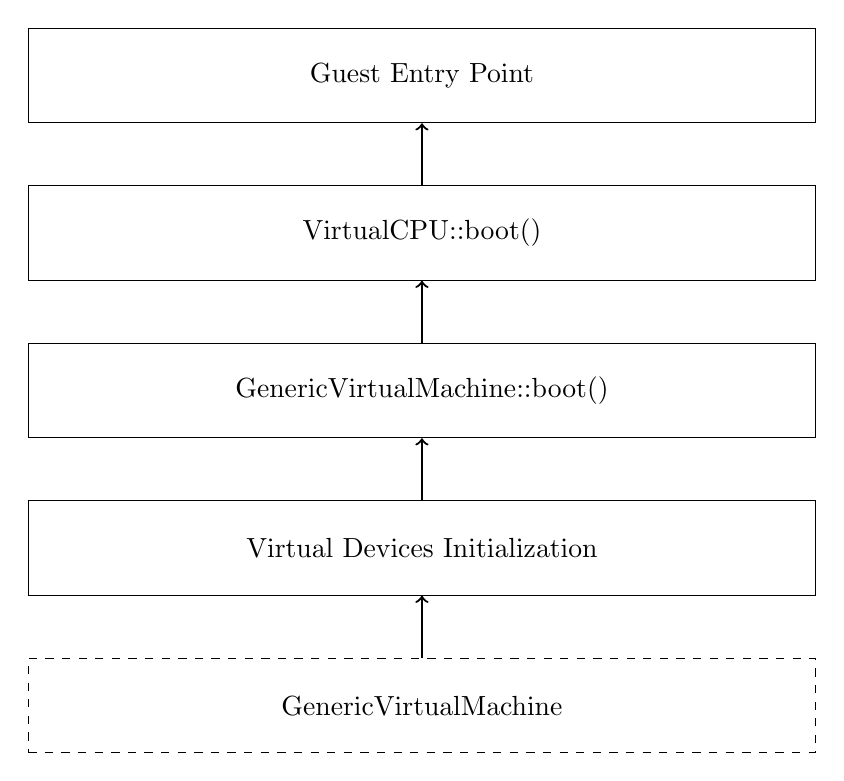
\begin{tikzpicture}
	        \node[rectangle, minimum width=10cm, minimum height=1.2cm, draw, align=center, dashed] (A) at (0,2){GenericVirtualMachine};
	        \node[rectangle, minimum width=10cm, minimum height=1.2cm, draw, align=center] (B) at (0,4){Virtual Devices Initialization};
	        \node[rectangle, minimum width=10cm, minimum height=1.2cm, draw, align=center] (C) at (0,6){GenericVirtualMachine::boot()};
	        \node[rectangle, minimum width=10cm, minimum height=1.2cm, draw, align=center] (D) at (0,8){VirtualCPU::boot()};
	        \node[rectangle, minimum width=10cm, minimum height=1.2cm, draw, align=center] (E) at (0,10){Guest Entry Point};
	        \draw[->, thick] (A) -- (B);
	        \draw[->, thick] (B) -- (C);
	        \draw[->, thick] (C) -- (D);
	        \draw[->, thick] (D) -- (E);
	    \end{tikzpicture}
	\end{center}
	\caption{Fluxo Geral de Inicialização de uma \textit{GenericVirtualMachine}.}
\end{figure}

%\subsection{\textit{VirtualCPU}: RISC-V}
%
%Para RISC-V, o processo de inicialização de uma CPU virtual é relativamente simples e pode ser descrito pelo fluxo apresentado
%na figura a seguir:
%
%\vspace{1cm}
%
%\begin{figure}[H]
%	\begin{center}
%	    \begin{tikzpicture}
%	        \node[rectangle, minimum width=10cm, minimum height=1.2cm, draw, align=center, dashed] (A) at (0,2){VirtualCPU::boot()};
%			\node[rectangle, minimum width=10cm, minimum height=1.2cm, draw, align=center] (B) at (0,4){Flush \gls{mmu} TLB};
%			\node[rectangle, minimum width=10cm, minimum height=1.2cm, draw, align=center] (C) at (0,6){Clear \glspl{csr}};
%			\node[rectangle, minimum width=10cm, minimum height=1.2cm, draw, align=center] (D) at (0,8){Set \gls{pmp} Registers};
%	        \node[rectangle, minimum width=10cm, minimum height=1.2cm, draw, align=center] (E) at (0,10){Delegate Interrupts};
%	        \node[rectangle, minimum width=10cm, minimum height=1.2cm, draw, align=center] (F) at (0,12){Delegate Exceptions};
%	        \draw[->, thick] (A) -- (B);
%	        \draw[->, thick] (B) -- (C);
%	        \draw[->, thick] (C) -- (D);
%	        \draw[->, thick] (D) -- (E);
%			\draw[->, thick] (E) -- (F);
%	    \end{tikzpicture}
%	\end{center}
%	\caption{Fluxo Geral de Inicialização de uma \textit{VirtualCPU} RISC-V.}
%\end{figure}
